\documentclass[tikz]{standalone}

\begin{document}

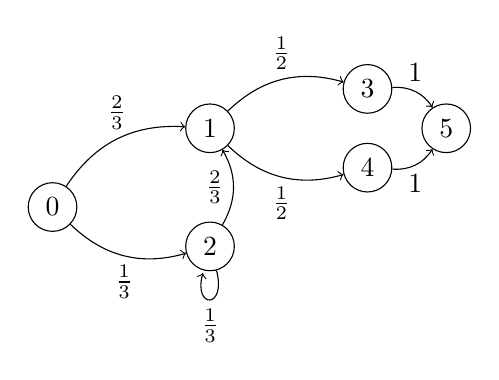
\begin{tikzpicture}
    \node [circle , draw ] (zero) at (0,0) {0};
    \node [circle , draw ] (one) at (2,1) {1};
    \node [circle , draw ] (two) at (2,-0.5) {2};
    \node [circle , draw ] (three) at (4,1.5) {3};
    \node [circle , draw ] (four) at (4,0.5) {4};
    \node [circle, draw ] (five) at (5,1) {5};
    \path[->] (two) edge [loop below] node {$\frac{1}{3}$} (two);
    \path[->] (zero) edge [bend left] node [above] {$\frac{2}{3}$} (one);
    \path[->] (zero) edge [bend right] node [below] {$\frac{1}{3}$} (two);
    \path[->] (one) edge [bend left] node [above] {$\frac{1}{2}$} (three);
    \path[->] (one) edge [bend right] node [below] {$\frac{1}{2}$} (four);
    \path[->] (three) edge [bend left] node [above] {$1$} (five);
    \path[->] (four) edge [bend right] node [below] {$1$} (five);
    \path[->] (two) edge [bend right] node [left] {$\frac{2}{3}$} (one);
\end{tikzpicture}
\end{document}
